\begin{figure}[hbtp]
  \centering
  \subfigure{
    \label{fig:about-auxiliary--with}
    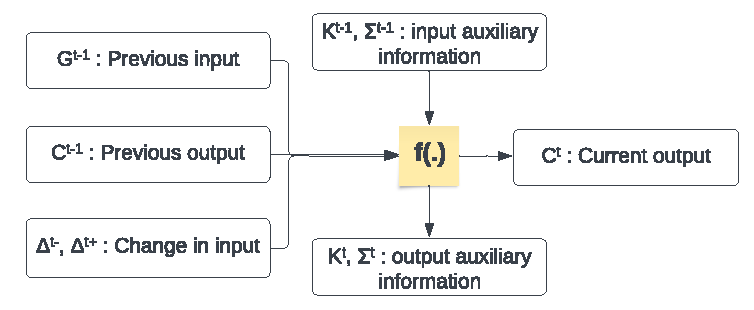
\includegraphics[width=0.98\linewidth]{out/about-auxiliary-with.pdf}
  } \\[-2ex]
  \caption{A dynamic community detection algorithm $f(.)$ takes as input the previous graph $G^{t-1}$, community memberships $C^{t-1}$, and the batch update $\Delta^{t-}$, $\Delta^{t+}$, and produces the updated community memberships $C^t$. However, it may also consider additional information such as the weighted degrees of vertices $K^{t-1}$ and the total edge weights of communities $\Sigma^{t-1}$ as auxiliary information, and yield updated auxiliary information $K^t$, $\Sigma^t$ \cite{sahu2024dflouvain}.}
  \label{fig:about-auxiliary}
\end{figure}
